\section{Method}
% too many "long-range dependencies"
In this research, we propose Conditional Self-attention Generative Adversarial Networks (CSGANs), which translate images from one domain to another being able to capture long-range dependencies and reserve the global structures across image. We first review the pix2pix model as our baseline (Sec. 3.1). And then we introduce the Conditional Self-attention Module (SCM) (Sec. 3.2). Finally, we describe the idea of multiple level patch discriminator and the loss we utilize to achieve this idea.
\subsection{Preliminary}
The pix2pix model [?] is an image-to-image translation framework based on conditional GANs, which trains a generator network $G$ and a discriminator network $D$. The generator $G$ takes as input conditional images and outputs corresponding target images, while the discriminator $D$ aims to distinguish real images from the synthesized ones. Formally, to train these two networks in a supervise manner, a set of pairs of corresponding images is required as training set $\{(x_i, y_i)\}$, where $x_i$ is a source image and $y_i$ is a corresponding target image. These two networks play a minmax game:
\begin{equation}
\label{eqn:minmax_game}
\min_G \max_D \mathcal{L}_{adv}(G,D)+\lambda \mathcal{L}_{L1}(G)
\end{equation}
to guide the generator to model the conditional distribution of real images given the source images, where the adversarial loss function is generally given by 
\begin{equation}
\label{eqn:loss_adv}
E_{(x,y)\sim p_{data}(x,y)}[\log D(x,y)]+E_{s\sim p_{data}(x)}[\log(1-D(x,G(x)))],
\end{equation}
and the $L_1$ loss is given by
\begin{equation}
\label{eqn:loss_l1}
\mathcal{L}_{L1}(G)=\mathbb{E}_{(x,y)\sim p_{data}(x,y)}[\|y-G(x)\|_1]
\end{equation}
The generator of pix2pix is a convolution-based U-Net \cite{Unet}. The condition image, the input of the generator, is only applied to the first layer. The discriminator is patch-wise discriminator introduced by PatchGANs \cite{PatchGANs}. The conditional image is concatenated channel-wisely to the synthesized image or real image as the input of the discriminator.
%
%
\begin{figure}
	\label{fig:CSM}
	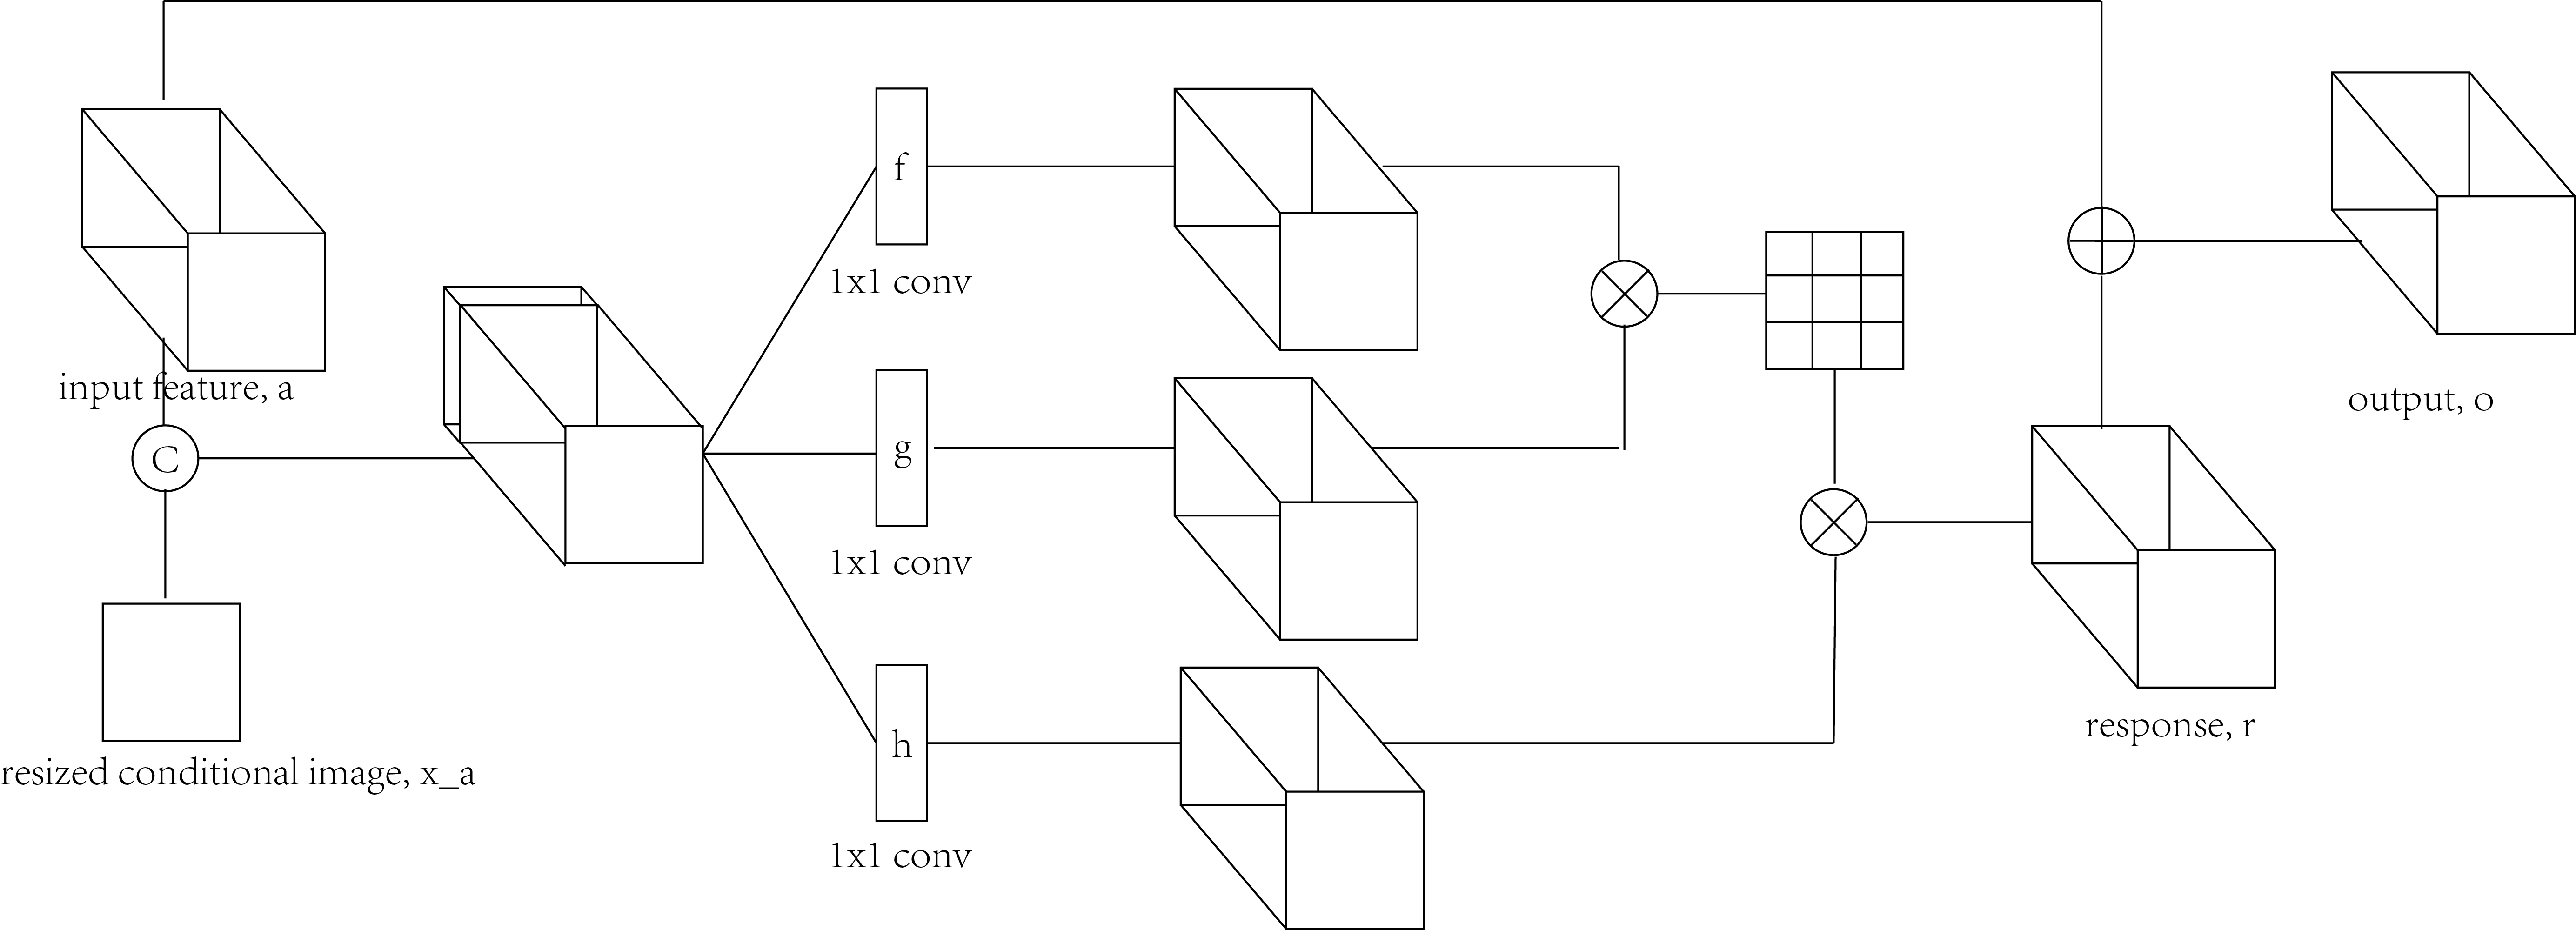
\includegraphics[width=0.8\textwidth]{figures/CSM}
	\caption{CSM}
\end{figure}
%
%
\subsection{Conditional Self-Attention Module (CSM)}
Since focusing on local receptive field, convolution operation has to establish a large receptive field through several layers, which is computationally inefficiently. It is possibly difficult for the optimizer to discover parameter values to model the relationship across the image. Inspired by \cite{non-local} and \cite{SAGANs}, we introduce a conditional self-attention module (CSM) to the convolution-based pix2pix framework in order to capturing the long-range dependencies of images and feature maps, as shown in Figure \ref{fig:CSM}
%

% $\boldmath{x} \bold{x} \mathbf{x} \mathbm{x} \vec{x}$
% TODO: notation of vectors and matrices, images and feature maps 
Given the image features from the previous hidden layer $a\in \mathbb{R}^{C\times M}$, we first resize the conditional image $x\in \mathbb{R}^{3\times N}$ to  $x_a\in \mathbb{R}^{3\times M}$ and concatenate the resized conditional image to the image feature to get $[a, x_a]$ as conditioned features, where $[\cdot,\cdot]$ is the concatenation operation. This allows the information of conditional image to convey to every attention module and guide the network to focuses on important regions directly based on the conditional image.
%
Then the conditioned features are mapped into three feature space by
\begin{equation}
\label{eqn:f}
f([a, x_a])=W_f[a, x_a],
\end{equation}
\begin{equation}
\label{eqn:g}
g([a, x_a])=W_g[a, x_a],
\end{equation}
\begin{equation}
\label{eqn:h}
h([a, x_a])=W_h[a, x_a],
\end{equation}
where $W_f, W_g\in \mathbb{R}^{\hat{C}\times (C+3)}$, $W_h\in \mathbb{R}^{(C+3)\times C}$ are trainable weights, which are implemented by $1\times 1$ convolutions. Here, we use $\hat{C}=C/16$ in our experiments. 
%
Let $\beta_{j,i}$ be the indicator that indicates the extent to which the model attends to the $i^{th}$ location when synthesizing the $j^{th}$ region, which is calculated by 
\begin{equation}
\label{eqn:beta}
\beta_{j,i}=\frac{exp(s_{ij})}{\sum^M_{i=1}exp(s_{ij})}
\end{equation}
where $s_{ij}=f([a, x_a])^Tg([a, x_a])$. Next, we use $\beta_{j,i}$ as the attention weights and compute the response $r=(r_1, r_2,\dot, r_M)\in \mathbb{R}^{\times M}$ at every position as a weighted sum of the features at all positions, where
\begin{equation}
\label{eqn:response}
o_j=\sum^M_{i=1}\beta_{j,i}h([a, x_a]).
\end{equation}
As suggested in \cite{SAGANs}, we further multiply the response of the attention layer by a scale parameter $\gamma$ and add back to the input feature maps. The final output is calculated by 
\begin{equation}
\label{eqn:output}
o_i=\gamma r_i+a_i,
\end{equation}
where $\gamma$ is trainable value and is set to $0$ at the beginning of the training process.This is because at the early stage of training process, the networks are able to learn the local dependencies, and then learn the long-range dependencies by assign more weight to the non-local evidence progressively.
%
%
\subsection{Multiple Level Patch Discriminator}
The discriminator pix2pix uses is a patch-wise dicriminator \cite{PatchGANs}, which distinguishes the real/synthesized images patch by patch with in a local receptive field much smaller than the size of the input images. 
The average value of all responses is provided as the ultimate output of $D$. 
This is based on the assumption of independence between pixels separated by more than a patch diameter. 
However, since the structure of every conditional image is global information across the entire image, the patch-wise discriminator may have troubles to capture this global information.
We add another global discriminator $D_g$ with a receptive field as large as the entire image to capture the global structure information. The patch discriminator $D_p$ and the global discriminator $D_g$ share weights in first few layers since the lower features of these discriminators should be the same, as shown in Figure \ref{fig:discriminators}.
%
%
\subsection{Architecture}
% add CSMs to discriminator or not? if not, why? (GPU memory budget limited)
Our architecture is based on the architecture of the pix2pix method which use a convolution-based U-Net \cite{Unet} as its generator and a patch-wise discriminator. We add the proposed CSM after every convolutional layers to the generator except the first and last ones. CSMs are able to access the information of the conditional image directly and model the long-range dependencies across images and feature maps. Also, we switch the patch-wise discriminator into the proposed multiple level patch discriminator to enable the discriminator network to capture both global and local information and therefore guide the generator to generator images with more structural layout.  
Figure \ref{fig:} shows the 
%
\begin{figure}
	\label{fig:architecture}
	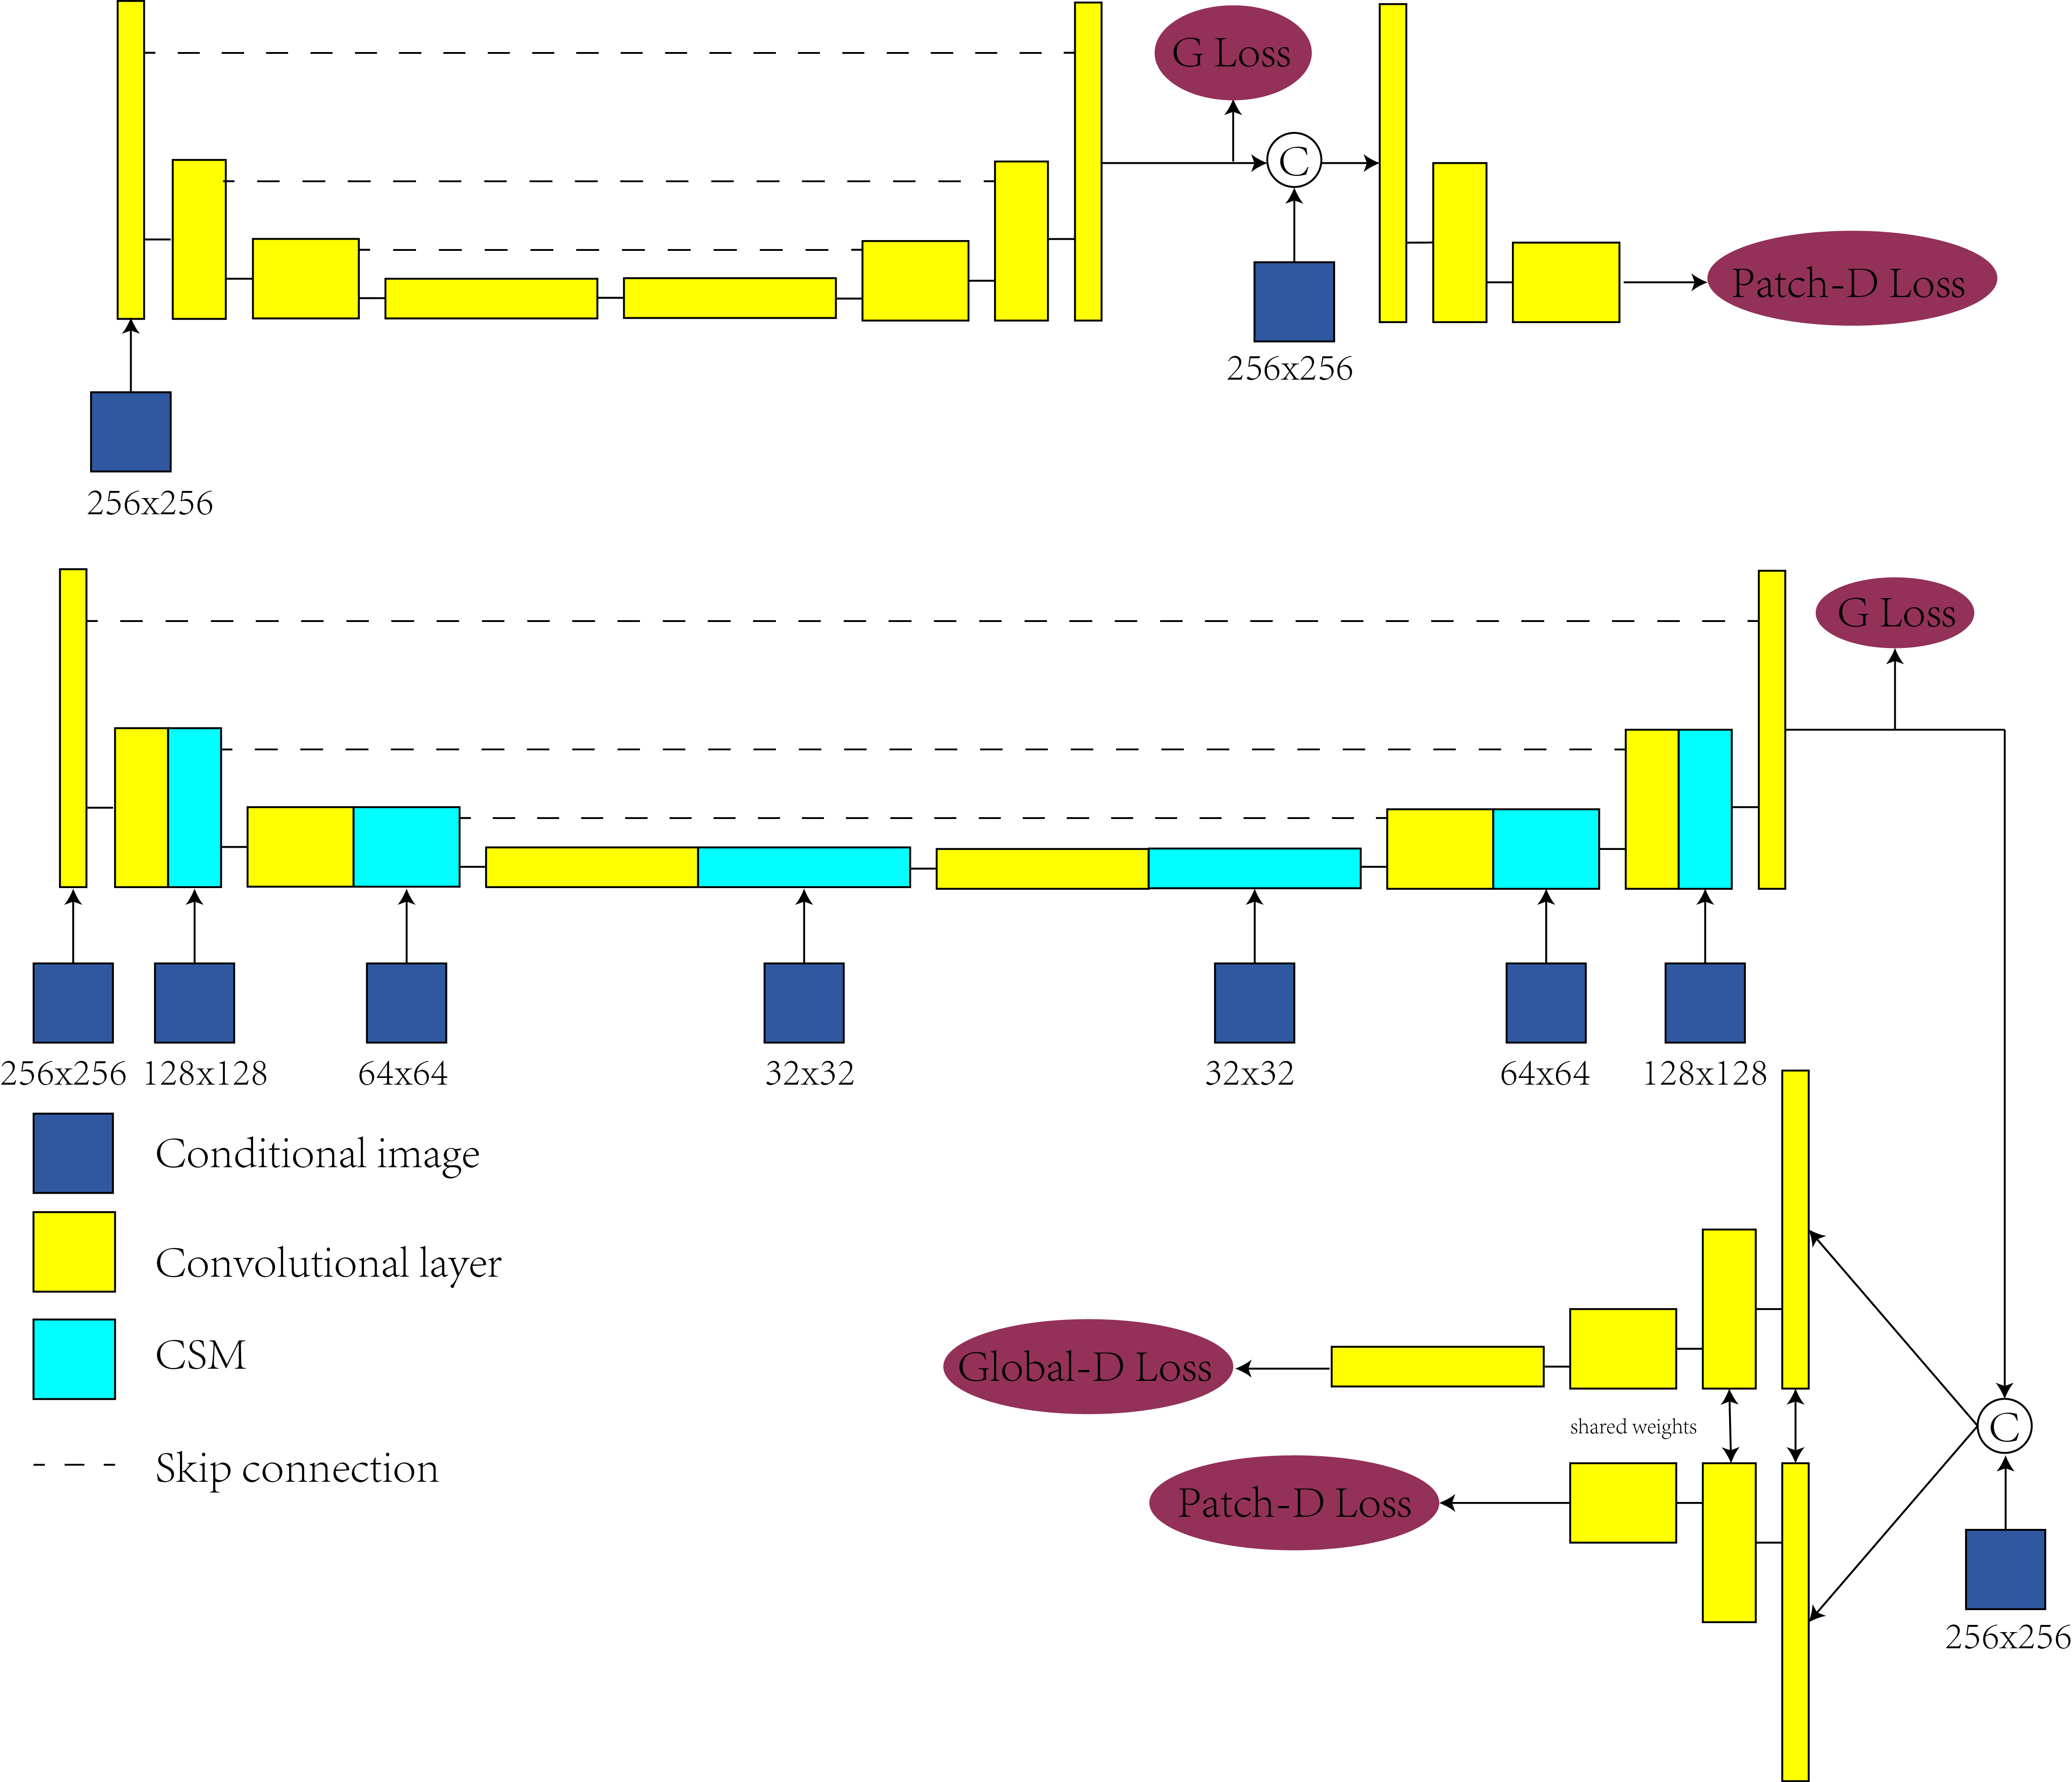
\includegraphics[width=0.8\textwidth]{figures/architecture}
	\caption{Architecure}
\end{figure}
%
\subsection{Other Techniques}
%
\paragraph{Noise vector} Some past conditional GANs add a noise vector to the generator as input to avoid it producing a deterministic output. However, the pix2pix model showed that the noise vector is just ignored by the generator network and not able to change the output samples. We observe the same phenomenon and do not apply the noise vector in our model. 
\paragraph{Spectral Normalization} Spectral normalization \cite{SN} is recently proposed normalization techniques, which restricts the spectral norm of each layer of the discriminator to constrain its Lipschitz constant. Spectral normalization is computationally efficient and require no extra hyper-parameter. It is shown that spectral normalization also benefit the training of generator by avoiding unusual gradients. We add spectral normalization to the discriminator and CSMs in the generator.
%